% ch3.tex
% This work is licensed under the Creative Commons Attribution-Noncommercial-Share Alike 3.0 New Zealand License.
% To view a copy of this license, visit http://creativecommons.org/licenses/by-nc-sa/3.0/nz
% or send a letter to Creative Commons, 171 Second Street, Suite 300, San Francisco, California, 94105, USA.


\chapter{Tartarugas e outras criaturas lentas}\index{Tartaruga}\label{ch:turtles}

Existem algumas similaridades entre as tartarugas do mundo real e a do Python. No mundo real, uma tartaruga é um réptil verde, que se move lentamente e carrega sua casa nas suas costas. No mundo do Python, uma tartaruga é uma pequena seta preta que se move lentamente pela tela. Sem se referir à uma casa nas costas.

De fato, considerando que a tartaruga do Python deixa uma trilha e se move pela tela, isso a torna menos parecida com uma tartaruga do mundo real e mais parecida com uma cobra, ou uma lesma. Porém, eu suponho que um módulo chamado `slug' (lesma) não seria muito atraente, então faz sentido continuar com as tartarugas. Imagine uma tartaruga carregando um par de pincéis e desenhando na tela conforme ela anda.

Em um passado profundo, escuro e distante, havia uma simples linguagem de programação chamada Logo. Logo foi usada para controlar uma tartaruga-robô (chamada Irving). Ao longo do tempo, a tartaruga evoluiu de um robô que se movia pelo chão, para uma pequena seta movendo pela tela.

\emph{O que só serve para mostrar que nem sempre as coisas melhoram conforme a tecnologia avança --- uma pequena tartaruga-robô seria muito mais divertido.}

O módulo `turtle' do Python (nós vamos chegar em módulos depois, mas por agora apenas imagine o módulo como algo que nós opdemos usar dentro de um programa) é um pouco como a linguagem de programação Logo, mas enquanto a Logo era (é) bem limitada, o Python possui muito mais recursos. O módulo `turtle' por si só, é um método muito útil para aprender como os computadores desenham figuras no seu monitor.

Vamos começar e ver como isso funciona. O primeiro passo, é dizer ao Python que nós queremos usar o módulo `turtle', importando-o:

\begin{listing}
\begin{verbatim}
>>> import turtle
\end{verbatim}
\end{listing}

Então nós precisamos exibir uma tela para desenhar. Uma tela parecida com a que os artistas usam para pintar; neste caso é um espaço branco para desenhar:

\begin{listing}
\begin{verbatim}
>>> tartaruga = turtle.Pen()
\end{verbatim}
\end{listing}

Nesse código, nós chamamos uma função (Pen\index{A função Pen}) do módulo `turtle', que automaticamente cria uma tela para nós desenharmos. Uma função é um pedaço de código reutilizável (nós veremos funções mais tarde) que faz algo útil --- neste caso, um objeto que representa uma tartaruga é retornado pela função `Pen' --- nós armazenamos esse objeto na variável `tartaruga'. Quando você digitar o código no terminal do Python, você verá uma tela em branco, assim como na figura~\ref{fig10}.

\begin{figure}
\begin{center}
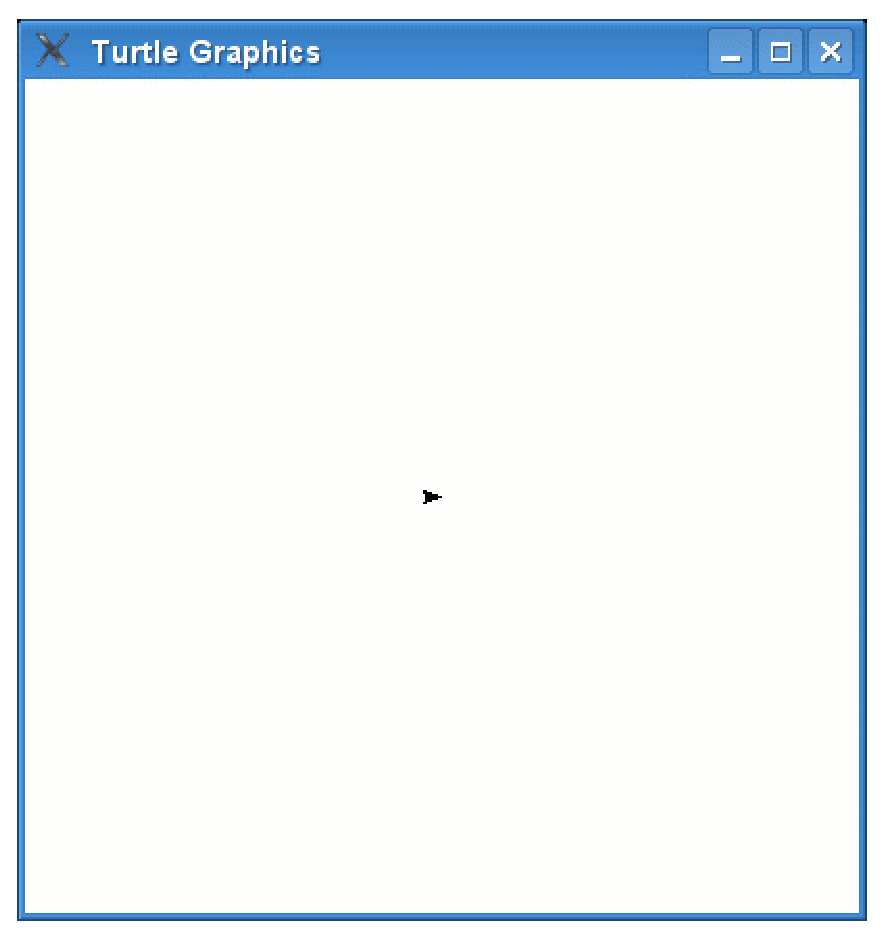
\includegraphics[width=72mm]{eps/figure10.eps}
\end{center}
\caption{Uma seta representando a tartaruga.}\label{fig10}
\end{figure}

\emph{Sim, aquela pequena seta no meio da tela é a nossa tartaruga. E, não, ela não se parece nenhum pouco com uma tartaruga.}

Você pode enviar instruções à tartaruga, usando algumas funções do objeto que nós criamos (chamando \code{turtle.Pen}) --- uma vez que nós atribuimos o objeto à variável \code{tartaruga}, nós usamos \code{tartaruga} para enviar instruções.

Uma das instruções é a \code{forward}. Forward (ir para frente, em inglês) diz à tartaruga para se mover para frente, seja qual for a direção que ela esteja. Vamos dizer à tartaruga para se mover 50 pixels para frente (nós falaremos sobre pixels em um minuto).

\begin{listing}
\begin{verbatim}
>>> tartaruga.forward(50)
\end{verbatim}
\end{listing}

Você verá algo como a figura ~\ref{fig11}.

\begin{figure}
\begin{center}
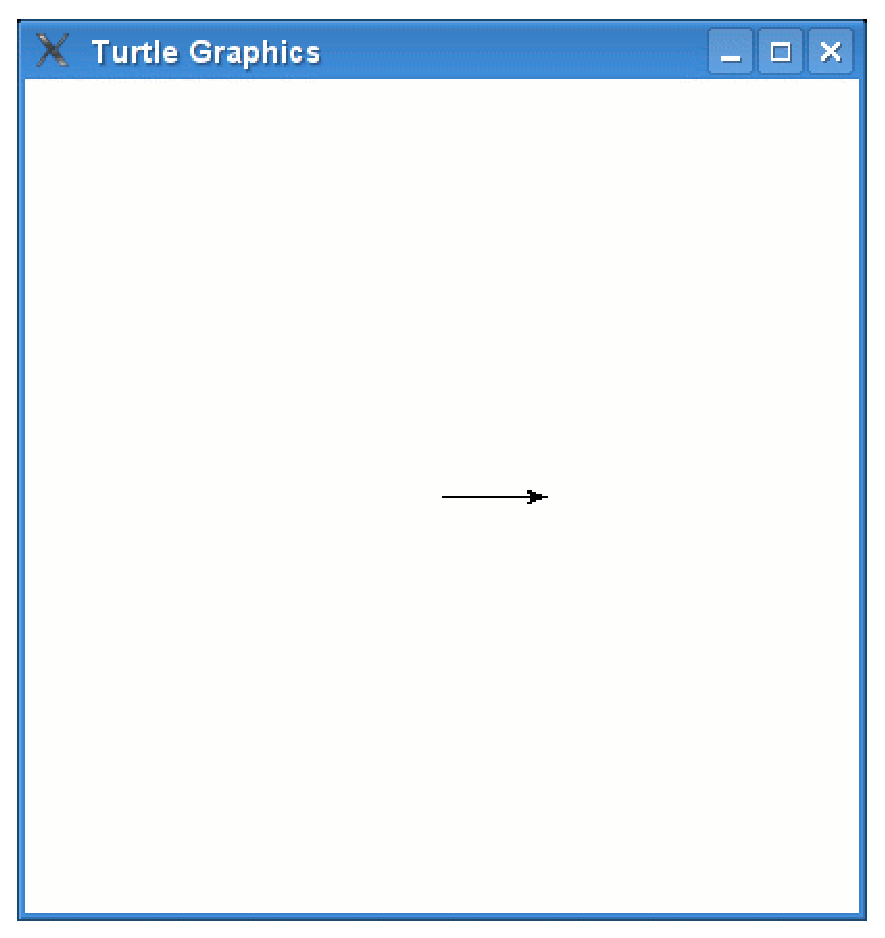
\includegraphics[width=72mm]{eps/figure11.eps}
\end{center}
\caption{A tartaruga desenha uma linha.}\label{fig11}
\end{figure}

Do ponto de vista da tartaruga, ela moveu 50 passos para frente. Do nosso ponto de vista, ela moveu 50 pixels.

\noindent
\emph{Então, o que é um pixel?}

Um pixel\index{Pixels} é um ponto na tela. Quando você olha para o seu computador, tudo é feito de pequenos pontos (quadrados). Os programas que você usa e os jogos que você joga no computador, ou com o seu PlayStation, ou Xbox, ou Wii; todos são formados por um monte de pontos coloridos diferentes, exibidos na tela. Na verdade, se você olhar para a tela do seu computador usando uma lente de aumento, você verá esses pontos. Então, se olharmos bem perto da linha desenhada pela tartaruga, nós veremos que a seta que representa a tartaruga, também é formata por um monte de pontos quadrados, como podemos ver na figura~\ref{fig12}.

\begin{figure}
\begin{center}
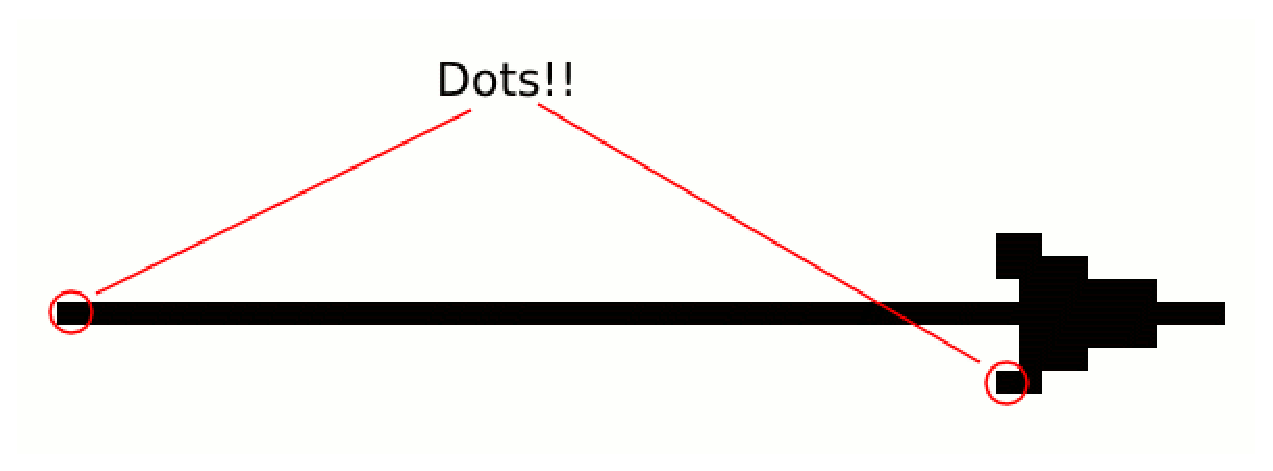
\includegraphics[width=72mm]{eps/figure12.eps}
\end{center}
\caption{Visão aproximada da linha e da seta.}\label{fig12}
\end{figure}

Nós falaremos mais tarde sobre esses pontos, ou pixels, em outro capítulo.

Depois, podemos dizer para a tartaruga virar para a esquerda\index{Tartaruga!vriando à esquerda} ou direita\index{Tartaruga!virando à direita}:

\begin{listing}
\begin{verbatim}
>>> tartaruga.left(90)
\end{verbatim}
\end{listing}

Isso diz à tartaruga para virar para a esquerda, 90 graus. Você pode não ter aprendido sobre graus\index{Graus} na escola ainda, mas uma maneira fácil de se pensar, é que eles são como as divisões em um relógio, assim como na figura~\ref{fig13}.

\begin{figure}
\begin{center}
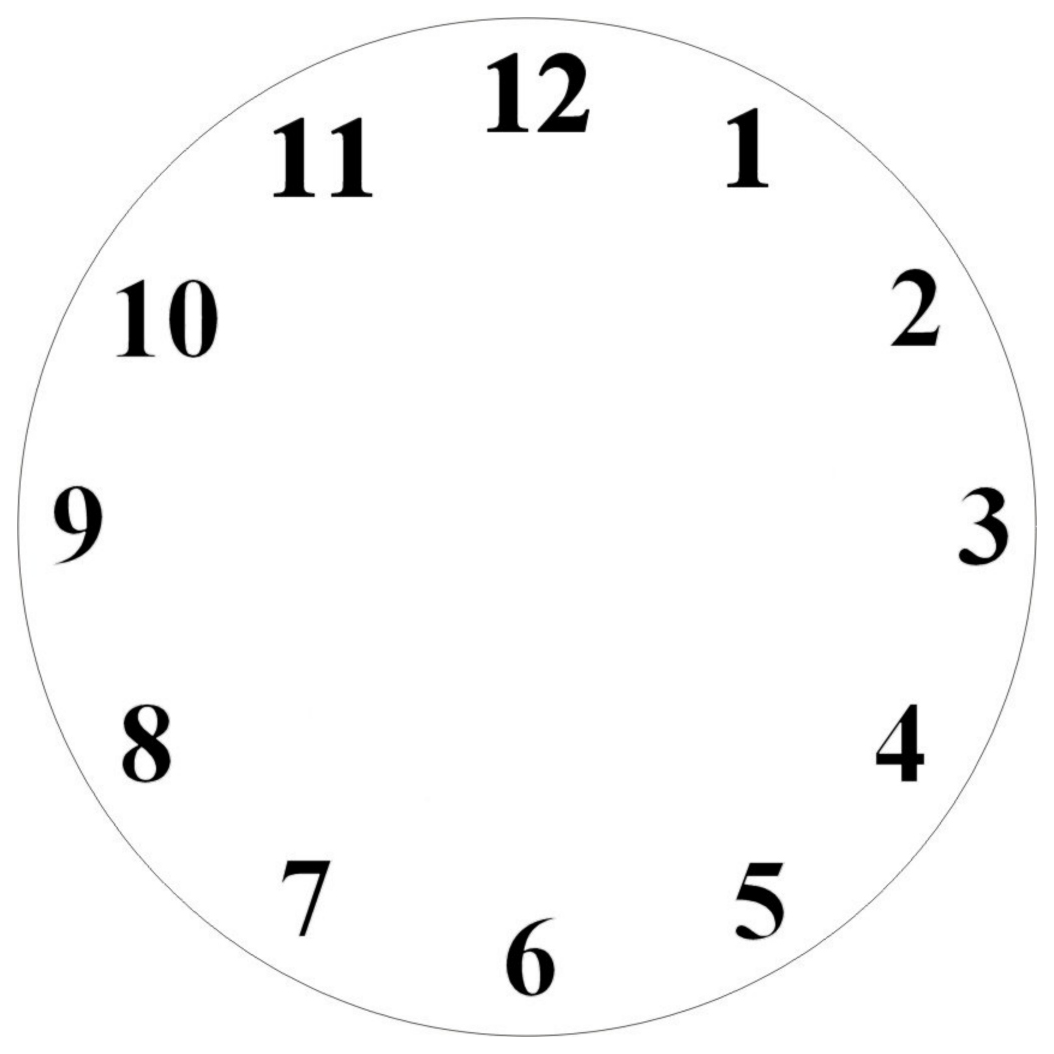
\includegraphics[width=52mm]{eps/figure13.eps}
\end{center}
\caption{As `divisões' em um relógio.}\label{fig13}
\end{figure}

A diferença de um relógio é que, ao invés de 12 divisões (ou 60, caso esteja contando em minutos ao invés de horas), existem 360 divisões. Então, se você contar as 360 divisões do relógio, você terá 90 onde marca 3 horas, 180 onde marca 6 horas e 270 onde marca 9 horas; e o 0, no começo, onde marca 12 horas. A figura~\ref{fig14} mostra as divisões em graus.

\begin{figure}
\begin{center}
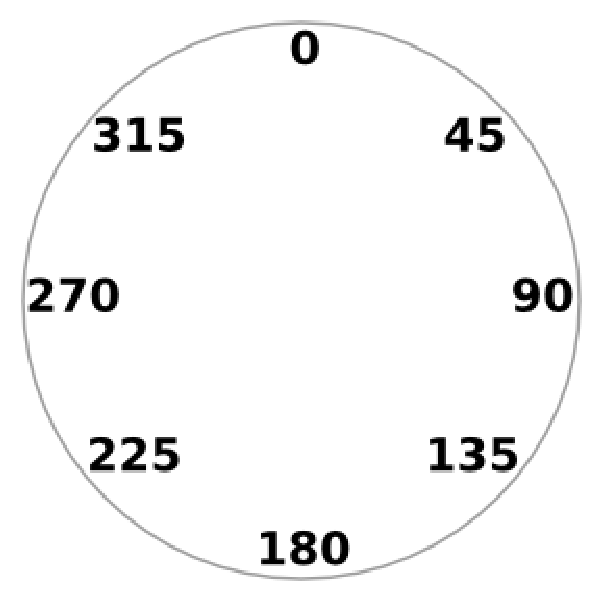
\includegraphics[width=52mm]{eps/figure14.eps}
\end{center}
\caption{Graus.}\label{fig14}
\end{figure}

Então, o que realmente significa quando você chama \code{left(90)}?
\par
Se você estender o seu braço para o lado, na direção do seu ombro, isso é 90 graus. Se você estender o seu braço esquerdo, isso é 90 graus para a esquerda. Se você estender o seu braço direito, isso é 90 graus para a direita. Quando a tartaruga do Python se vira à esquerda, ela posiciona o seu rosto para a esquerda e então gira o seu corpo para a nova direção (da mesma forma que você faria para saber para onde o seu braço está apontando). Então, \code{tartaruga.left(90)} faz com que a seta agora aponte para cima, como exibido na figura~\ref{fig15}.

\begin{figure}
\begin{center}
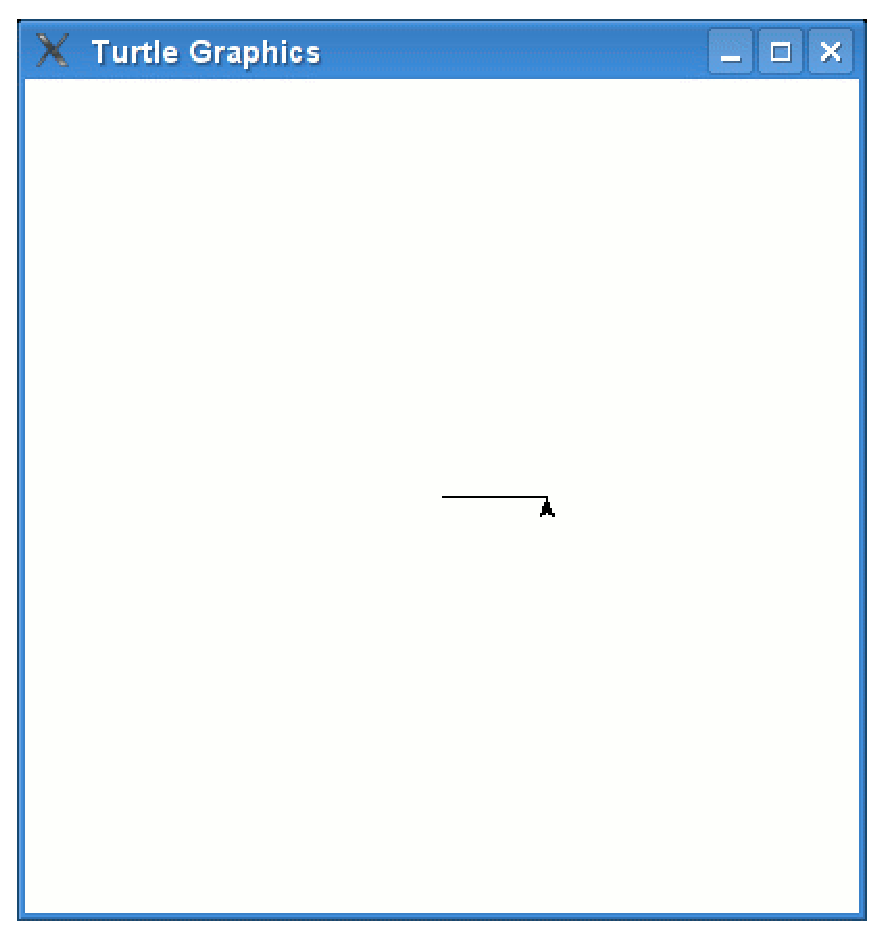
\includegraphics[width=72mm]{eps/figure15.eps}
\end{center}
\caption{A tartaruga, após virar para a esquerda.}\label{fig15}
\end{figure}

Vamos tentar os mesmos comandos novamente, algumas vezes:

\begin{listing}
\begin{verbatim}
>>> tartaruga.forward(50)
>>> tartaruga.left(90)
>>> tartaruga.forward(50)
>>> tartaruga.left(90)
>>> tartaruga.forward(50)
>>> tartaruga.left(90)
\end{verbatim}
\end{listing}

Nossa tartaruga desenhou um quadrado e ficou virada para a mesma direção que estava (veja a figura~\ref{fig16}).

\begin{figure}
\begin{center}
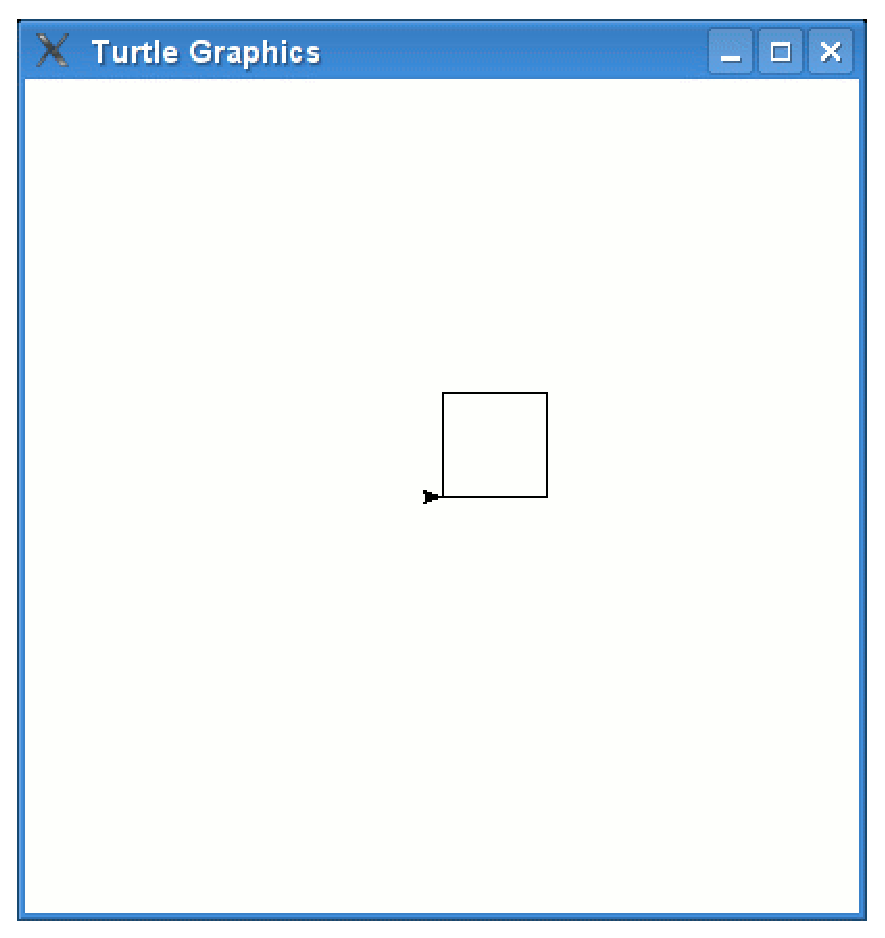
\includegraphics[width=72mm]{eps/figure16.eps}
\end{center}
\caption{Desenhando um quadrado.}\label{fig16}
\end{figure}

Nós podemos limpar o que está na tela, usando o comando clear\index{Tartaruga!Limpando}:

\begin{listing}
\begin{verbatim}
>>> tartaruga.clear()
\end{verbatim}
\end{listing}

Algumas das outras funções básicas que você pode usar são: \code{reset}\index{Tartaruga!Recomeçando}, que também limpa a tela, mas também coloca a tartaruga de volta na sua posição inicial; \code{backward}\index{Tartaruga!Indo para trás}, que move a tartaruga para trás; \code{right}, que vira a tartaruga para a direita; \code{up}\index{Tartaruga!Indo para frente} que diz à tartaruga para parar de desenhar conforme ela anda (como se tirasse o pincel da tela); e finalmente o \code{down}\index{Tartaruga!Indo para baixo} que diz à tartaruga para voltar a desenhar. Você pode chamar essas funções da mesma forma que chamou as outras:

\begin{listing}
\begin{verbatim}
>>> tartaruga.reset()
>>> tartaruga.backward(100)
>>> tartaruga.right(90)
>>> tartaruga.up()
>>> tartaruga.down()
\end{verbatim}
\end{listing}

\noindent
Nós voltaremos ao módulo `turtle' em breve.

\section{Coisas para tentar}

\emph{Neste capítulo, nós vimos como usar o módulo `turtle' para desenhar linhas simples, virando-a para esquerda e direita. Nós vimos que são usados graus para virar a tartaruga, um pouco parecido com as divisões dos minutos em um relógio.}.

\subsection*{Exercício 1}
Crie uma tela usando a função \code{Pen} do módulo `turtle' e desenhe um retângulo.

\subsection*{Exercício 2}
Crie outra tela usando a função \code{Pen} e desenhe um triangulo.

\newpage
